\documentclass[tikz,border=1mm]{standalone}
\usepackage{amsmath,amssymb}
\usepackage{xcolor}
\definecolor{cblue}{RGB}{59,130,246}
\definecolor{cgray}{RGB}{148,163,184}
\definecolor{cgreen}{RGB}{34,197,94}
\definecolor{corange}{RGB}{249,115,22}
\definecolor{arrow}{RGB}{148,163,184}
\usetikzlibrary{arrows.meta,calc}

\begin{document}
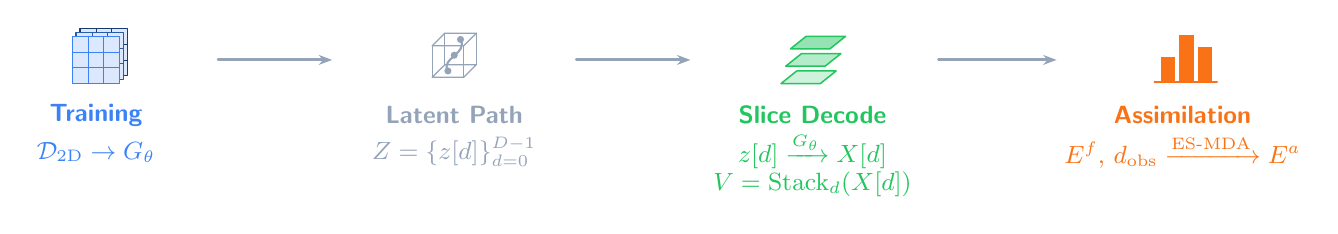
\begin{tikzpicture}[
    line cap=round,
    line join=round,
    >={Stealth[length=1.7mm,width=1.25mm]},
    arr/.style={->, line width=1.05pt, draw=arrow},
    title/.style={font=\sffamily\bfseries\small},
    formula/.style={font=\small},
  ]

  \begin{scope}[shift={(0,0)}]
    \begin{scope}[shift={(0,0.55)}]
      \foreach \dx/\dy/\op in {0.10/0.10/45, 0.05/0.05/70, 0.00/0.00/100}{
        \draw[line width=0.55pt, cblue!\op!black, fill=cblue!18]
          (-0.30+\dx,-0.30+\dy) rectangle (0.30+\dx,0.30+\dy);
        \draw[line width=0.28pt, cblue!\op!black]
          (-0.30+\dx,-0.10+\dy) -- (0.30+\dx,-0.10+\dy)
          (-0.30+\dx,0.10+\dy) -- (0.30+\dx,0.10+\dy)
          (-0.10+\dx,-0.30+\dy) -- (-0.10+\dx,0.30+\dy)
          (0.10+\dx,-0.30+\dy) -- (0.10+\dx,0.30+\dy);
      }
    \end{scope}
    \node[title, text=cblue] at (0,-0.15) {Training};
    \node[formula, text=cblue] at (0,-0.62) {$\mathcal{D}_{2\mathrm{D}}\to G_{\theta}$};
  \end{scope}

  \begin{scope}[shift={(4.55,0)}]
    \begin{scope}[shift={(0,0.55)}]
      \draw[line width=0.45pt, cgray]
        (-0.28,-0.22) -- (0.12,-0.22) -- (0.28,-0.06) -- (-0.12,-0.06) -- cycle;
      \draw[line width=0.45pt, cgray]
        (-0.28,0.18) -- (0.12,0.18) -- (0.28,0.34) -- (-0.12,0.34) -- cycle;
      \draw[line width=0.45pt, cgray]
        (-0.28,-0.22) -- (-0.28,0.18)
        (0.12,-0.22) -- (0.12,0.18)
        (0.28,-0.06) -- (0.28,0.34)
        (-0.12,-0.06) -- (-0.12,0.34);
      \draw[line width=0.75pt, cgray]
        (-0.08,-0.14) .. controls (-0.18,0.02) and (0.18,0.08) .. (0.08,0.26);
      \fill[cgray] (-0.08,-0.14) circle (0.045);
      \fill[cgray] (0.00,0.06) circle (0.045);
      \fill[cgray] (0.08,0.26) circle (0.045);
    \end{scope}
    \node[title, text=cgray] at (0,-0.15) {Latent Path};
    \node[formula, text=cgray] at (0,-0.62) {$Z=\{z[d]\}_{d=0}^{D-1}$};
  \end{scope}

  \begin{scope}[shift={(9.10,0)}]
    \begin{scope}[shift={(0,0.55)}]
      \draw[line width=0.55pt, cgreen, fill=cgreen!22]
        (-0.40,-0.30) -- (0.10,-0.30) -- (0.30,-0.14) -- (-0.20,-0.14) -- cycle;
      \draw[line width=0.55pt, cgreen, fill=cgreen!34]
        (-0.34,-0.08) -- (0.16,-0.08) -- (0.36,0.08) -- (-0.14,0.08) -- cycle;
      \draw[line width=0.55pt, cgreen, fill=cgreen!48]
        (-0.28,0.14) -- (0.22,0.14) -- (0.42,0.30) -- (-0.08,0.30) -- cycle;
    \end{scope}
    \node[title, text=cgreen] at (0,-0.15) {Slice Decode};
    \node[formula, text=cgreen, align=center] at (0,-0.78)
      {$z[d]\xrightarrow{G_{\theta}}X[d]$\\[-1pt]
       $V=\mathrm{Stack}_{d}(X[d])$};
  \end{scope}

  \begin{scope}[shift={(13.80,0)}]
    \begin{scope}[shift={(0,0.55)}]
      \fill[corange] (-0.28,-0.28) rectangle (-0.10,0.04);
      \fill[corange] (-0.04,-0.28) rectangle (0.14,0.32);
      \fill[corange] (0.20,-0.28) rectangle (0.38,0.16);
      \draw[line width=0.45pt, corange] (-0.36,-0.28) -- (0.44,-0.28);
    \end{scope}
    \node[title, text=corange] at (0,-0.15) {Assimilation};
    \node[formula, text=corange] at (0,-0.62)
      {$E^{f},\,d_{\mathrm{obs}}\xrightarrow{\mathrm{ES\text{-}MDA}}E^{a}$};
  \end{scope}

  \draw[arr] (1.55,0.55) -- (3.00,0.55);
  \draw[arr] (6.10,0.55) -- (7.55,0.55);
  \draw[arr] (10.70,0.55) -- (12.20,0.55);

\end{tikzpicture}
\end{document}
